Tady se zkusíme podívat, jak by mohl být veden důkaz hypotézy \ref{hyp:ofcitnumu} -- O funkci tnumu.

\begin{remind}
Hypotéza O funkci tnumu propojovala pojem funkce tnumu a precizního operátoru. Vztah v ní obsažený je syntakticky jednoduchý:
\begin{equation}
\mathcal{T}^{f(x)}(\varepsilon)=[\mathcal{T}^x]^{f, \varepsilon}_\infty
\end{equation}
a předpokládá existenci libovolně přesné funkce pro racionální číslo, postupným iterováním precizního operátoru pak rozšiřujeme definiční obor na libovolné reálné číslo, které má tnum.
\end{remind}

Trochu si teď tento vztah rozepišme. Bez použití notace tnumu a precizního operátoru se snažíme dokázat, že
\begin{equation}
f\left(x+\frac{\varepsilon}{f\left(x+\frac{\varepsilon}{f\left(x+\frac{\varepsilon}{\ldots}\right)}\right)}\right)\in[f(x)-\varepsilon, f(x)+\varepsilon ]
\end{equation}
a také
\begin{equation}
f\left(x-\frac{\varepsilon}{f\left(x-\frac{\varepsilon}{f\left(x-\frac{\varepsilon}{\ldots}\right)}\right)}\right)\in[f(x)-\varepsilon, f(x)+\varepsilon ],
\end{equation}
také jakékoli jiné pořadí znamének, ne jen $+,+,+,+,\ldots$ a $-,-,-,-,\ldots$ ale také $+,-,+,-,\ldots$ atp.

Podotkněme, že při implementaci je podmínka rekurze rovnost dvou po sobě jdoucích členů posloupnosti precizního operátoru. Při výpočtu funkce se pak hledí na předchozí funkční hodnotu (dříve to nešlo, protože tnumy jsou líné) a o ni se upravuje přesnost argumentu.

Nejprve se zkusme zamyslet, jaký důkaz použijeme. Všechny důkazy matematiky tnumů byly \textit{přímé důkazy}, dokazovali jsme vztahy dobře zachytitelné na papír a vlastně šlo jen o odvození. Tady ale nemáme jednoznačně danou levou stranu, protože díky rekurzivnímu zápisu ji ani nelze zachytit, natož rozepsat a dokázat. Oblíbený je též \textit{důkaz sporem}, ten se ale používá u očividných tvrzení a negací předpokladu pak odvodíme nějaký protimluv. Toto tvrzení ale nevypadá tak očividně, ikdyž jsem o jeho správnosti přesvědčen. Ani sporem tedy dokazovat nebudeme. Jak už bylo řečeno, precizní operátor je posloupnost a pravdy o posloupnostech se dokazují \textit{induktivně}. Narážíme ale na problém, jak zformulovat indukční předpoklad. Víme totiž, že pro členy, které jsou různé od svého předchůdce nebudou naši podmínku splňovat a dokazujeme až skutečnost, že se někdy členy začnou rovnat a že tato hodnota je opravdu naše hledaná. Tedy ani klasickou matematickou indukcí to asi nepůjde.

Podívejme se nyní, jak vypadá situace na nějaké klesající spojité funkci.
\begin{myfigure}{H}
\caption{Nultá iterace precizního operátoru}
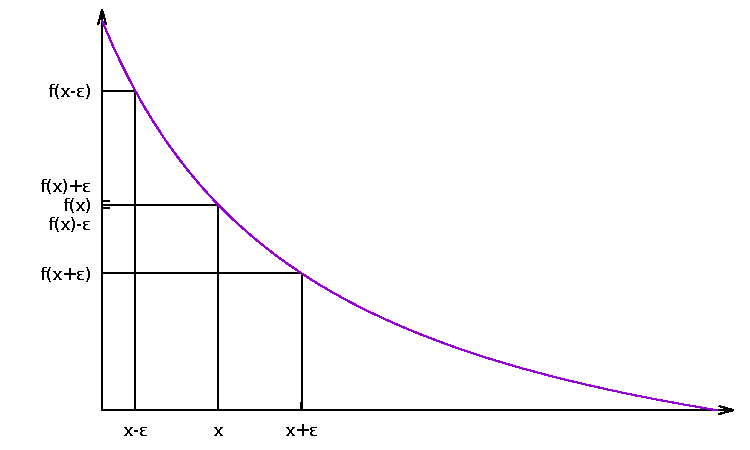
\includegraphics[width=\linewidth]{graphics/obr1.pdf}\label{fig:obr1}
Rozdíl mezi $f(x)+\varepsilon$ a $f(x+\varepsilon)$ na funkci $1/x$ v bodě $x=0.2$, $\varepsilon=0.05$.
\end{myfigure}
Intervaly se zúží, když uděláme první otočku precizního operátoru.
\begin{myfigure}{H}
\caption{První iterace precizního operátoru}
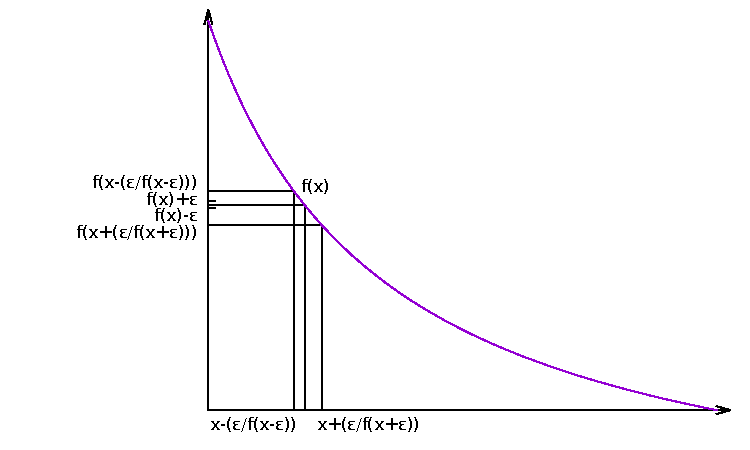
\includegraphics[width=\linewidth]{graphics/obr2.pdf}\label{fig:obr1}
Znázornění zlepšení přesnosti, když místo $f(x+\varepsilon)$ vezmeme $f\left(x+\frac{\varepsilon}{f(x+\varepsilon)}\right)$.
\end{myfigure}
Nepřekvapivě to funguje, ikdyž prohodíme znaménka.
\begin{myfigure}{H}
\caption{První iterace precizního operátoru}
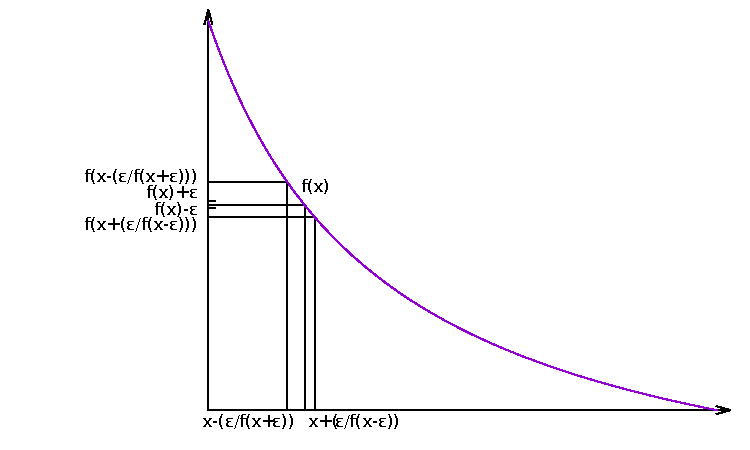
\includegraphics[width=\linewidth]{graphics/obr3.pdf}\label{fig:obr1}
I $f\left(x+\frac{\varepsilon}{f(x-\varepsilon)}\right)$ je lepší než $f(x+\varepsilon)$. Podobně pro $f\left(x-\frac{\varepsilon}{f(x+\varepsilon)}\right)$.
\end{myfigure}

Další otočka už je na zobrazení grafem docela oříšek, protože už máme 8 funkčníh hodnot podle různých znamének. V tomto případě jsou nejkrajnější body $f\left(x+\frac{\varepsilon}{f\left(x+\frac{\varepsilon}{f(x+\varepsilon)}\right)}\right)$ a $f\left(x-\frac{\varepsilon}{f\left(x+\frac{\varepsilon}{f(x+\varepsilon)}\right)}\right)$, ve dříve nastolené notaci trojice $\langle+, +, +, \rangle$ a $\langle-, +, +\rangle$.